\chapter{Identificação e Refactoring de Code Smells}
\hspace{5mm} Neste capítulo identificam-se os diferentes \emph{code smells} presentes no código fornecido pela equipa docente e os respetivos tratamentos efetuados (refactoring).

\section{Bloaters}
\hspace{5mm} Nesta secção apresentam-se os diferentes tipos de \emph{Bloaters} encontrados. Um \emph{code smell Bloater} consiste em código, métodos e classes de grandes proporções, dificultando a sua análise.

\subsection{Data Clumps}
\hspace{5mm} Os \emph{Data Clumps} ocorrem quando grupos de variáveis ocorrem repetitivamente ao longo do código. Desta forma, no código fornecido, nas classes \emph{DAO} verificou-se a repetição de uma variável \textbf{c} do tipo \emph{Connection} em todas os métodos, tal como se pode observar na figura \ref{img:data-cumpls-1}.

\hspace{5mm} Assim, o tratamento realizado a este \emph{code smell}, foi a declaração desta variável \textbf{c}, como variável de instância da classe \textbf{AtivoDAO} e a colocação de um nome mais intuitivo para a variável, como \textbf{connection}, tal como se pode observar na figura \ref{img:data-cumpls-2}. 

\hspace{5mm} O \emph{code smell}, ocorre em todas as classes \emph{DAO}, ou seja, o tratamento vai ser aplicado a todas.

\begin{figure}[H]
	\centering
	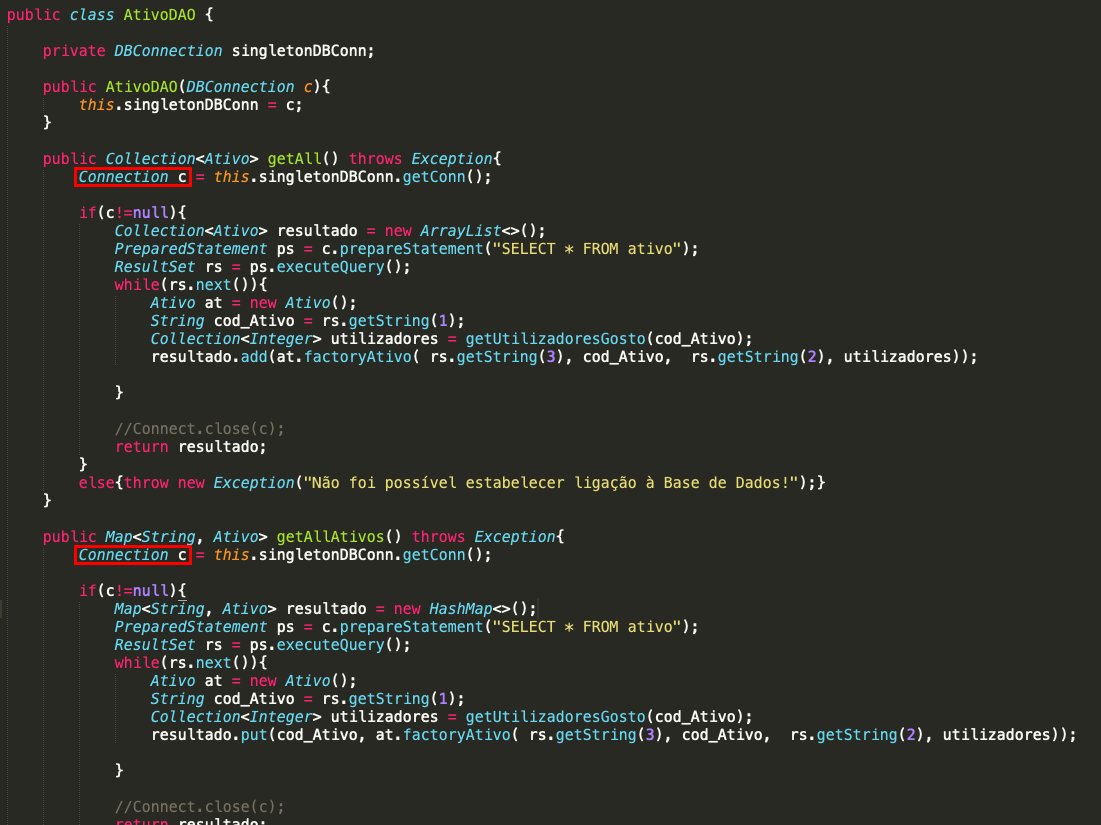
\includegraphics[scale=0.35]{images/bloaters/data-clumps/b1-1.png}
	\caption{Repetição da variável \textbf{c} to tipo \emph{Connection} em todos os métodos.}
	\label{img:data-cumpls-1}
\end{figure}

\begin{figure}[H]
	\centering
	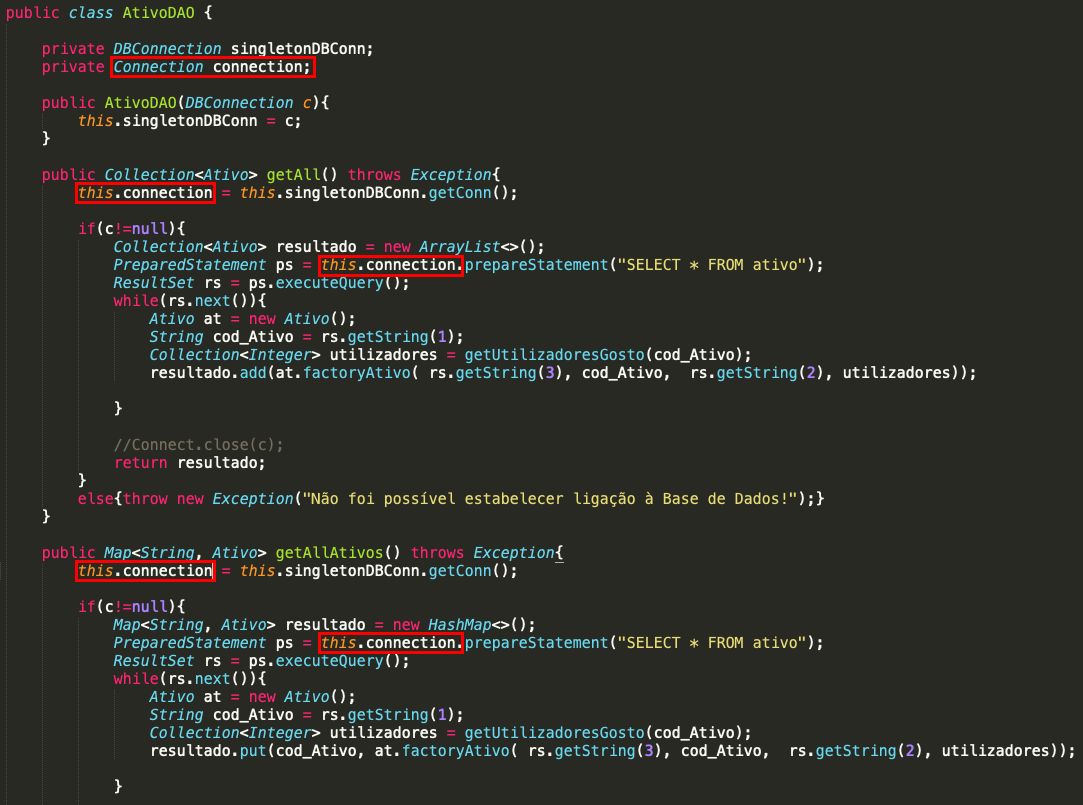
\includegraphics[scale=0.35]{images/bloaters/data-clumps/b1-2.png}
	\caption{Tratamento realizado ao \emph{code smell} data clumbs da categoria Bloaters.}
	\label{img:data-cumpls-2}
\end{figure}

\subsection{Long Method}

\begin{figure}[H]
	\centering
	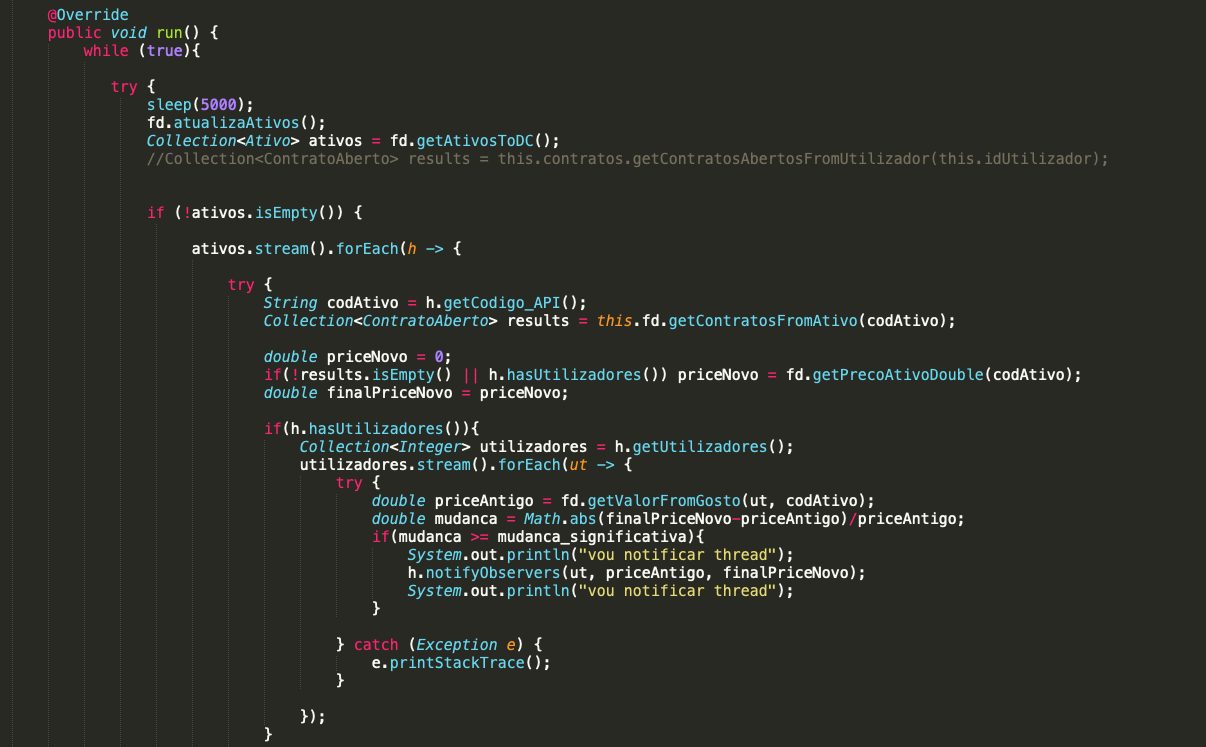
\includegraphics[scale=0.40]{images/bloaters/long-method/b2-1-1.png}
	\label{img:long-method-1}
\end{figure}

\begin{figure}[H]
	\centering
	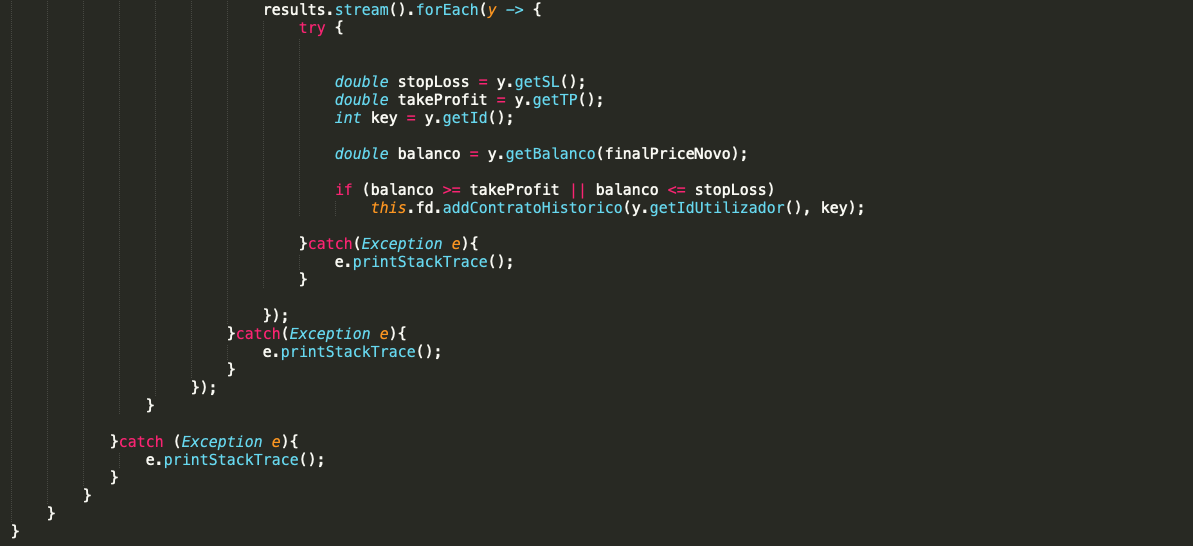
\includegraphics[scale=0.40]{images/bloaters/long-method/b2-1-2.png}
	\caption{Um método com 67 linhas.}
	\label{img:long-method-2}
\end{figure}

\hspace{5mm} O \emph{code smell} identificado na figura \ref{img:long-method-2}, consiste num método que contém mais de dez linhas de código, dificultando a sua leitura e dessa forma a sua análise. 

\hspace{5mm} Assim, o tratamento para este \emph{code smell}, denomina-se \emph{Extract Method}, consiste em distribuir diferentes partes/funcionalidades do método, em métodos auxiliares mais simples, e com responsabilidades distintas, reduzindo assim, o seu tamanho e facilitando a sua análise. Deste modo, foram criados três métodos auxiliares e removidas/renomeadas certas variáveis que não fariam sentido.

\hspace{5mm} No bloco de código, que ficou no método \textbf{verificarPrecoAtivosSeguidos}, verificou-se que estava a ser usada um variável desnecessária, denominada \textbf{finalPriceNovo}, deste modo, a mesma foi removida.

\begin{figure}[H]
	\centering
	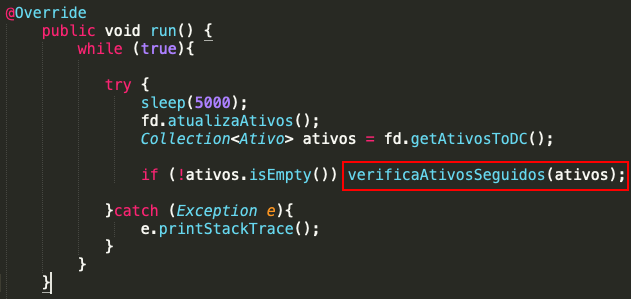
\includegraphics[scale=0.65]{images/bloaters/long-method/b2-2-1.png}
	\caption{Método run\(\) simplificado.}
	\label{img:pag}
\end{figure}

\begin{figure}[H]
	\centering
	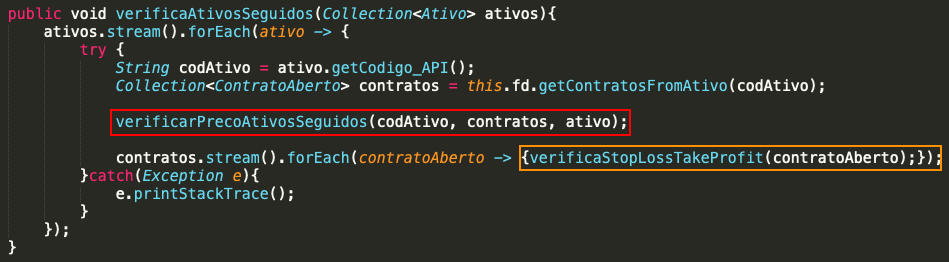
\includegraphics[scale=0.55]{images/bloaters/long-method/b2-2-2.png}
	\caption{Método auxiliar, que por sua vez chama os outros métodos auxiliares.}
	\label{img:pag}
\end{figure}

\begin{figure}[H]
	\centering
	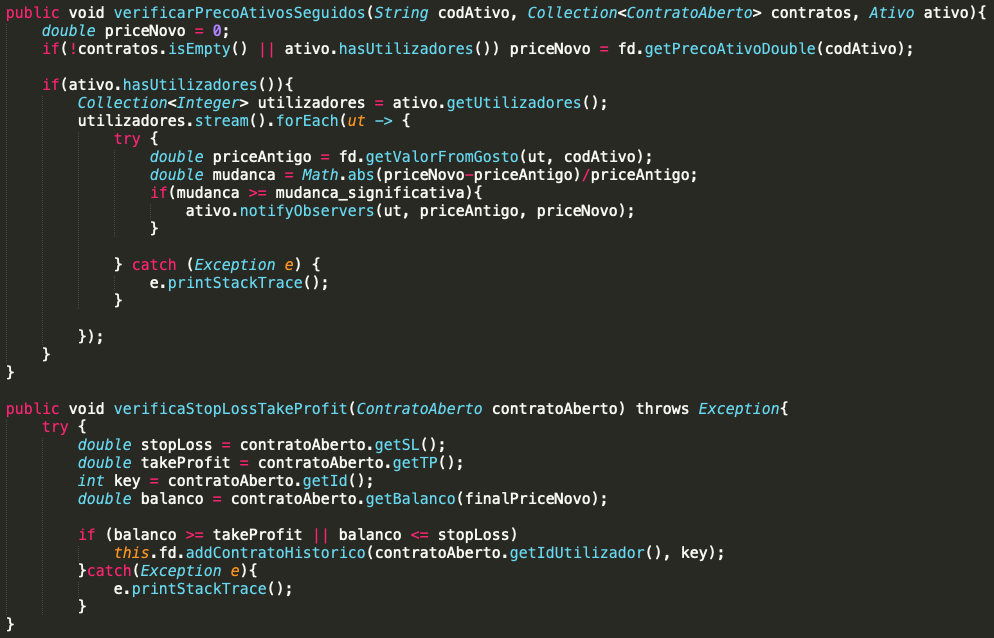
\includegraphics[scale=0.45]{images/bloaters/long-method/b2-2-3.png}
	\caption{Métodos auxiliares chamados no método \textbf{verificarAtivosSeguidos}.}
	\label{img:pag}
\end{figure}

\subsection{Long Parameter List}

\hspace{5mm} O \emph{code smell} identificado consiste em métodos com mais de quatro argumentos. Desta forma, encontrou-se um método, denominado \textbf{addContratoPortfolio}, na class \textbf{Facade}, do package \textbf{Negócio}, que tem mais de quatro argumentos, tal como se pode observar na figura \ref{img:long-parameter-1}. 

\begin{figure}[H]
	\centering
	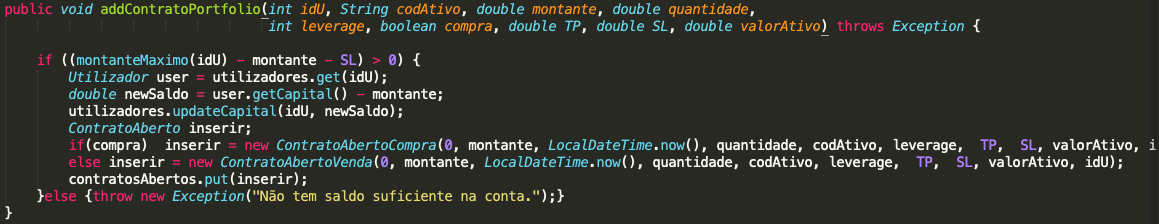
\includegraphics[scale=0.45]{images/bloaters/long-parameters/long-parameters-1.png}
	\caption{Método com mais de quatro argumentos.}
	\label{img:long-parameter-1}
\end{figure}

\hspace{5mm}Deste modo, como se trata de uma adição do contrato ao portfolio, o tratamento a efetuar denomina-se \emph{Introduce Parameter Object}, ou seja, como o objeto \textbf{Contrato} contém quase todas as variáveis enviadas como argumento, excepto o \emph{StopLess} \- SL, \emph{Take Profit} \-TP e o tipo de contrato, \emph{Compra} ou \emph{Venda}, então envia-se o objeto \emph{Contrato}, e as variáveis que faltam neste, tal como se pode observar na figura \ref{img:long-parameter-2}.

\hspace{5mm} Neste tratamento também foi aplicado a técnica \emph{Extrat Variable}, visto que as variáveis \textbf{quantidade}, \textbf{montante}, entre outras, são utilizadas mais do que uma vez, compensando guardar o valor das mesmas numa variável temporária, para que não se chame repetitivamente o método \emph{get} dessas variáveis. 

\hspace{5mm} Importante realçar que, ainda se podia ter feito um melhor tratamento, mas devido à hierarquia do \textbf{Contrato}, não estar correta, pois tal como se irá abordar mais adiante, não era necessário a diferenciação entre contratos abertos ou fechados, ou de compra e venda através de classes, pois estes vários tipos ou derivações de contratos, mantém as mesmas variáveis. 

\hspace{5mm} Na verdade, o correto na opinião do grupo, será diferenciar estes tipos, com a utilização de variáveis na classe \textbf{Contrato} e dessa forma, este método apenas precisaria de receber o objeto \textbf{Contrato}. Isto é, bastava colocar na classe \textbf{Contrato} um variável boolean, que identifica se o contrato é de compra ou venda, e outra variável boolean, que identifica se o contrato está aberto ou fechado.

\begin{figure}[H]
	\centering
	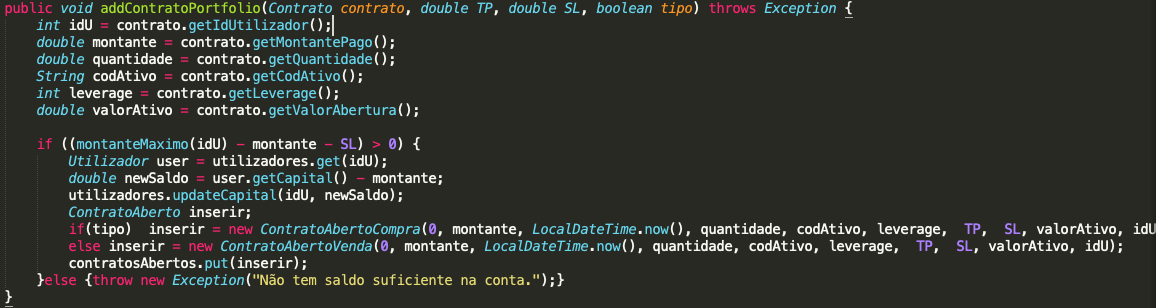
\includegraphics[scale=0.45]{images/bloaters/long-parameters/long-parameters-2.png}
	\caption{Método reduzido para 4 argumentos.}
	\label{img:long-parameter-2}
\end{figure}

\newpage
\section{Object-Orientation Abusers}
Nesta secção apresentam-se os diferentes tipos de \emph{code smells} desta categoria. Um \emph{Object-Orientation Abusers} consiste na aplicação incorreta ou incompleta dos princípios de programação orientada a objetos.

\subsection{Design pattern observer incorretamente implementado}

\hspace{5mm} Verificou-se que a equipa não implementou o \emph{design pattern} \emph{observer} da melhor forma.

\hspace{5mm} Este \emph{design pattern} consiste num objeto (Observable) notificar outro (Observer), através do método \textbf{notifyObservers()}. A equipa que desenvolveu o código implementou essa lógica, no entanto \textbf{especificou todos os parâmetros} que são enviados na notificação para o Observer. Desta forma, caso sejam necessários enviar mais parâmetros, facilmente o método notifyObservers() fica com uma \textbf{lista desnecessariamente aumentada de parâmetros}, tornando-se num \emph{code smell} denominado de \emph{Long Parameter List}, tal como a seguinte figura ilustra.

\begin{figure}[H]
	\centering
	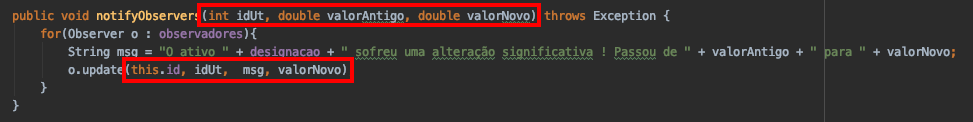
\includegraphics[scale=0.55]{images/design_pattern_observer_before.png}
	\caption{Incorreta especificação dos parâmetros referentes ao Ativo no método notifyObservers.}
	\label{img:pag}
\end{figure}

\hspace{5mm} Acrescentando, ao especificar os parâmetros (neste caso sobre o Ativo) torna a reutilização da interface impossível (que vai contra um dos princípios de POO) uma vez que o código não é genérico. Desta forma propõe-se a alteração da lista de parâmetros específicos ao Ativo, para apenas um único argumento do tipo Object, tornando o \emph{design pattern} genérico e possível de reutilizar as interfaces várias vezes ao longo do projeto ou mesmo noutros projetos, tal como se apresenta de seguida. 

\begin{figure}[H]
	\centering
	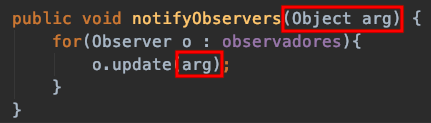
\includegraphics[scale=0.55]{images/design_pattern_observer_after_1.png}
	\caption{Modificação dos parâmetros para um único argumento genérico do tipo Object.}
	\label{img:pag}
\end{figure}

\hspace{5mm} Desta forma a evocação do método notifyObservers() também sofreu alterações para introduzir a forma mais genérica, antes o método era evocado da forma, como se pode ver na figura \ref{img:pag1}.

\begin{figure}[H]
	\centering
	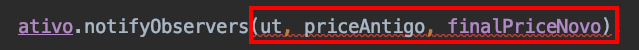
\includegraphics[scale=0.55]{images/design_pattern_observer_before_2.png}
	\caption{Evocação do método notifyObservers antes da modificação.}
	\label{img:pag1}
\end{figure}

\hspace{5mm} Para corrigir a modificação, cria-se um array de objetos contendo os parâmetros e envia-se os mesmos como um único objeto, tal como se pode observar na figura \ref{img:pag2}.

\begin{figure}[H]
	\centering
	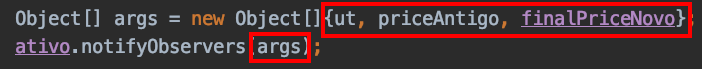
\includegraphics[scale=0.55]{images/design_pattern_observer_after_2.png}
	\caption{Evocação do método notifyObservers após a modificação.}
	\label{img:pag2}
\end{figure}

\subsection{Classe com a responsabilidade errada}

\hspace{5mm} Na classe Ativo verificou-se que a variável \textbf{utilizadores} não faz sentido existir, uma vez que não é da responsabilidade da classe Ativo guardar a lista de utilizadores que seguem um determinado ativo, pois o comportamento de seguir um ativo é realizado pelo utilizador.

\hspace{5mm} Note-se que o código é funcionalmente correto, no entanto um dos princípios de POO é colocar o comportamento (métodos) e variáveis na classe que tem a responsabilidade em causa. Por isso, entendeu-se que a variável utilizadores deve ser removida da classe Ativo e na classe \textbf{Utilizador} deve ser introduzida a variável \textbf{ativos}, que contém a lista de ativos que o utilizador segue, tal como as figuras \ref{img:pag3} e \ref{img:pag4} ilustram.

\begin{figure}[H]
	\centering
	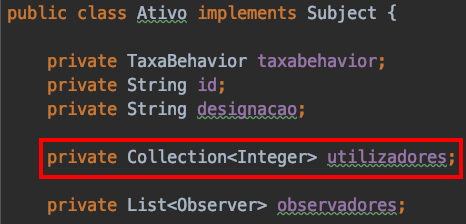
\includegraphics[scale=0.55]{images/POO_abuser_before_1.png}
	\caption{Variável utilizadores removida da classe Ativo.}
	\label{img:pag3}
\end{figure}

\begin{figure}[H]
	\centering
	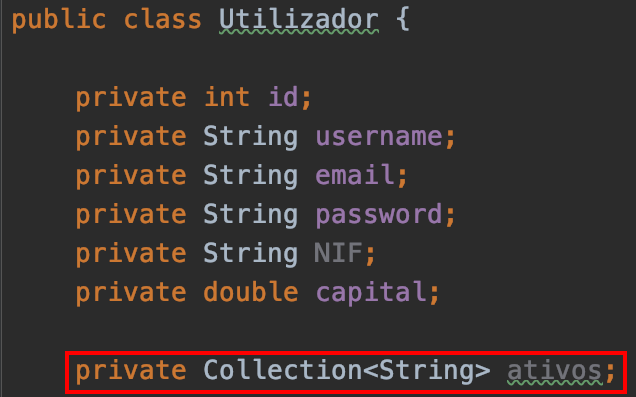
\includegraphics[scale=0.40]{images/POO_abuser_after_1.png}
	\caption{Variável ativos introduzida na classe Utilizador.}
	\label{img:pag4}
\end{figure}

\newpage
\section{Change Preventers \& Couplers}
\hspace{5mm} O \emph{Change Preventers} ocorre quando a necessidade de uma alteração numa parte do código, cria a necessidade de se alterar também em muitas outras partes.

\hspace{5mm} O \emph{Couplers} ocorre quando existe acoplamento excessivo entre classes, ou em alternativa a este, excessiva delegação.

\hspace{5mm} A razão pela qual se juntou estes dois \emph{code smells}, deve-se ao facto, de ambos estarem relacionados, isto é, quando um ocorre, o outro provavelmente também. Desta forma, os exemplos encontrados verificam ambos, devido ao facto, por exemplo, acoplamento em excesso, dificultar alterações no futuro.

\subsection{Shotgun Surgery}

\hspace{5mm} Em relação a \emph{code smells} destas categorias, a equipa que desenvolveu o código não seguiu corretamente a noção de package, divisão de responsabilidades e redução das dependências. 

\hspace{5mm} Na verdade, o package \textbf{DataObject}, não tem uma classe \textbf{Facade}, isto é, uma classe que expõe as funcionalidades deste package, encapsulando o interior do mesmo. A vantagem deste encapsulamento, é a redução das dependências entre os packages, permitindo alterações no futuro, sem a necessidade de mudar outros packages ou classes que usem estas funcionalidades.

\hspace{5mm} Na figura \ref{img:change-prevents-1}, verifica-se a presença destes \textit{code smells}, isto é, a dependência de classes internas do package \textbf{DataObject}, na classe \textbf{Facade} do package \textbf{Negócio}, que poderia ser facilmente evitada, com a utilização de uma classe \textbf{FacadeDataObject} no package \textbf{DataObject}. 

\hspace{5mm} Assim, se no futuro, fosse necessário mudar totalmente a forma como o package \textbf{DataObject} funciona, isto é, as suas classes (por exemplo o nome das mesmas, ou serem substituídas por outras), a classe \textbf{Facade} do package \textbf{Negócio}, entre outras, também teriam que ser mudadas.

\hspace{5mm} Desta forma, o tratamento a realizar, e como já foi referido, consiste na criação de uma classe no package \textbf{DataObject}, que exponha as funcionalidades do package, encapsulando o interior do mesmo. De seguida,  adiciona-se essa classe, como variável de instância da classe \textbf{Facade} do package \textbf{Negócio}, tal como se pode observar na figura \ref{img:change-prevents-2}.

\begin{figure}[H]
	\centering
	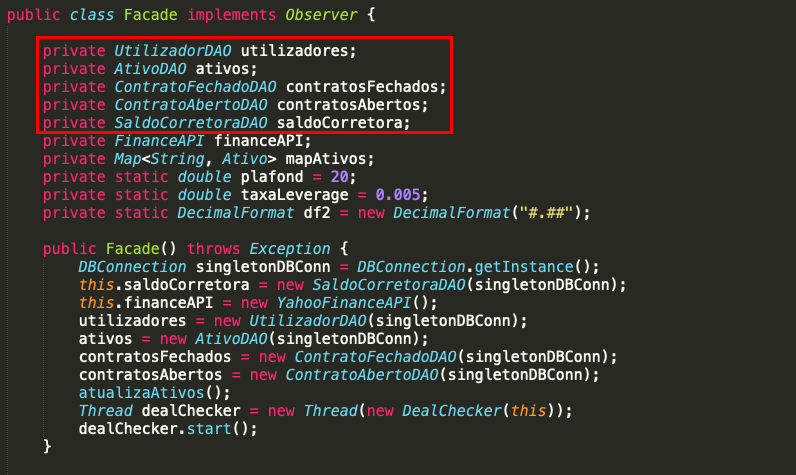
\includegraphics[scale=0.50]{images/change-prevents/change-prevents-1.png}
	\caption{Classe com várias dependências com o package \emph{DataObject}}
	\label{img:change-prevents-1}
\end{figure}

\begin{figure}[H]
	\centering
	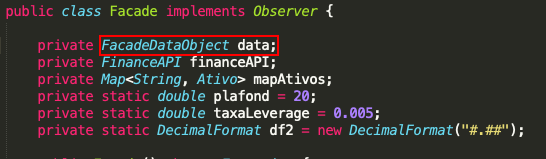
\includegraphics[scale=0.70]{images/change-prevents/change-prevents-2.png}
	\caption{Classe com apenas uma dependência em relação ao package \textbf{DataObject}.}
	\label{img:change-prevents-2}
\end{figure}

\subsection{Design pattern factory incorretamente implementado}

\hspace{5mm} O \emph{design pattern} Factory Method é utilizado para fabricar objetos de um determinado tipo através de uma interface mais geral, sendo possível produzir diferentes sub-tipos dos mesmos objetos através das respetivas sub-classes. A  grande  vantagem  deste  \emph{design  pattern} é a \textbf{eliminação de dependências com  as várias sub-classes}. No caso da classe Ativo caso se pretendesse introduzir mais N sub-classes da mesma, mantinha-se apenas as duas dependências (com a interface IAtivo e a classe FactoryAtivo) ao invés de o número de dependências aumentar em N. 

\hspace{5mm} Posto isto, verificou-se que o propósito do \emph{design pattern} não foi de todo respeitado com a implementação atual do código, uma vez que o método de criação do Ativo encontra-se exatamente na mesma classe (Ativo), sendo incorreto, pois este devia estar definido numa classe à parte denominada de FactoryAtivo e é necessário a existência de uma interface IAtivo. Desta forma, o propósito de reduzir o número de dependências não é impossível de atingir, não existindo, na prática, a implementação do \emph{design pattern}, consequentemente aumentado o acoplamento entre as várias classes que usam a classe Ativo.

\hspace{5mm} Conclui-se que o \emph{refactoring}, neste caso, seria mais dispendioso do que simplesmente deixar a versão atual implementado, uma vez que a própria arquitetura em geral teria de ser alterada, introduzidas interfaces para cada tipo de dados (Ativo, Utilizador e cada tipo de contratos) e não só implementar o design pattern para a classe Ativo como para as restantes.

\newpage
\section{Dispensables}

\hspace{5mm} \emph{Dispensables} consiste no código ou documentação que não faz sentido existir ou a ausência do mesmo torna mais eficiente e facilitada a compreensão do código.

\hspace{5mm} Na classe Utilizador verificou-se que a variável NIF não é utilizada tal como a figura \ref{img:pag5} ilustra.

\begin{figure}[H]
	\centering
	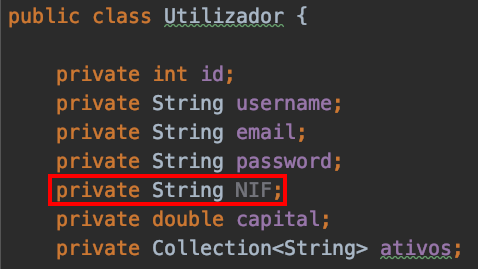
\includegraphics[scale=0.55]{images/dispensable_1.png}
	\caption{Variável NIF não é utilizada na classe Utilizador.}
	\label{img:pag5}
\end{figure}

\hspace{5mm} Ainda na mesma classe verificou-se que 6 métodos, 1 getter e 5 setters, não estavam a ser utilizados tal como se pode observar na figura \ref{img:pag6}.

\begin{figure}[H]
	\centering
	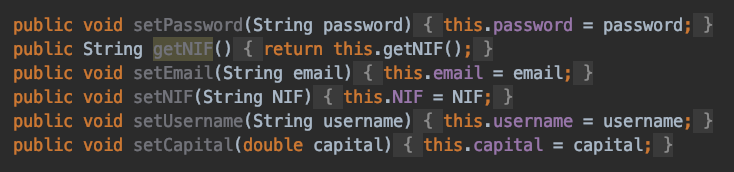
\includegraphics[scale=0.55]{images/dispensable_2.png}
	\caption{6 métodos não são utilizados na classe Utilizador.}
	\label{img:pag6}
\end{figure}

\hspace{5mm} Note-se que, apesar dos métodos não serem utilizados, as variáveis (à excepção do NIF) são utilizadas, por exemplo no construtor. Acrescentando, apesar de no final do trabalho os métodos acabaram por não ser utilizados, tem sentido a sua criação inicial uma vez que é um bom princípio de POO, no momento de criação de uma variável também serem criados os métodos getters e setters, pois podem ser utilizados no futuro.

\newpage
\section{Outros}
Nesta secção apresentam-se \emph{code smells}, que não tem uma categoria específica, mas que são considerados.

\subsection{Nome da variável não intuitivo}

\hspace{5mm} No desenvolvimento do código, por vezes não se escolhe o nome mais intuitivo para descrever o propósito de uma variável. Apesar do código ser funcionalmente correto, torna mais difícil a compreensão futura do mesmo, e até a própria pessoa que o desenvolveu pode ter dificuldades.

\hspace{5mm} Na figura \ref{img:pag7}, a variável \textbf{codigo\_API} refere-se ao identificador da classe Ativo, sendo que o nome mais apropriado poderia ser \textbf{id}. Note-se que ao se chamar \textbf{codigo\_API} implicitamente está a indicar que utilizou uma API para obter o Ativo, e por isso não existe abstração de implementação (um dos princípios de POO) e até mesmo porque a classe Ativo pode ser reutilizada para outro projeto (outro príncipio de POO) e deve ser o mais genérica possível sendo que não deve ser alusiva ao uso de uma API. Por outro lado, um \textbf{código} pode ser usado para variados propósitos, sendo que deve ser especificado que é o código \textbf{identificador}. 

\begin{figure}[H]
	\centering
	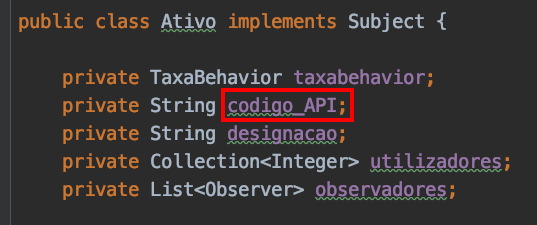
\includegraphics[scale=0.55]{images/change_variable_name_before.png}
	\caption{Variável codigo\_API na classe Ativo.}
	\label{img:pag7}
\end{figure}


\begin{figure}[H]
	\centering
	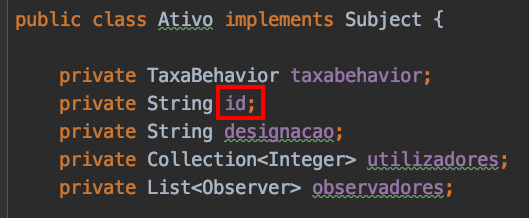
\includegraphics[scale=0.55]{images/change_variable_name_after.png}
	\caption{Modificação do nome para id.}
	\label{img:pag}
\end{figure}

\hspace{5mm} Na classe DealChecker, responsável por encerrar contratos CFD, reparou-se que cada ativo era denominado por \textbf{h} o que, em primeira análise, não se entendeu ao que esta variável se referia, tal como se pode observar na figura \ref{img:pag8}.

\begin{figure}[H]
	\centering
	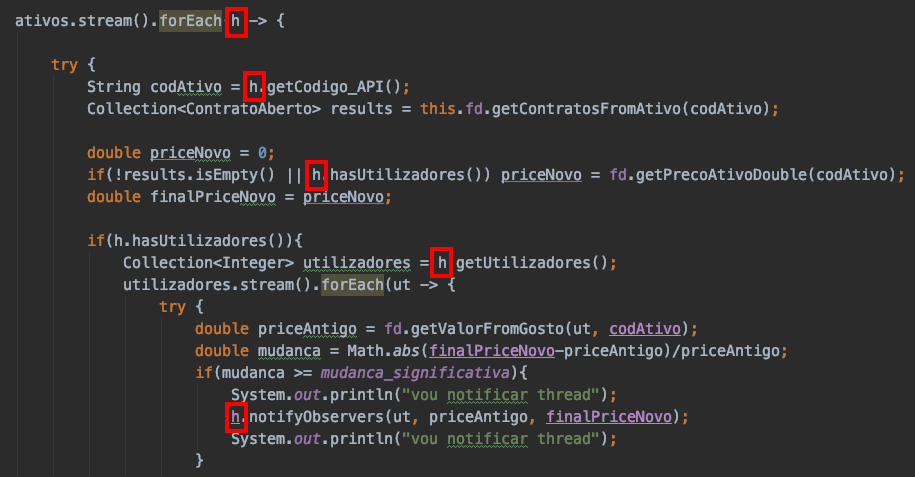
\includegraphics[scale=0.55]{images/change_variable_name_before_2.png}
	\caption{Variável h na classe DealChecker.}
	\label{img:pag8}
\end{figure}

\hspace{5mm} A simples mudança do nome da variável tornou o código mais fácil de se entender.

\begin{figure}[H]
	\centering
	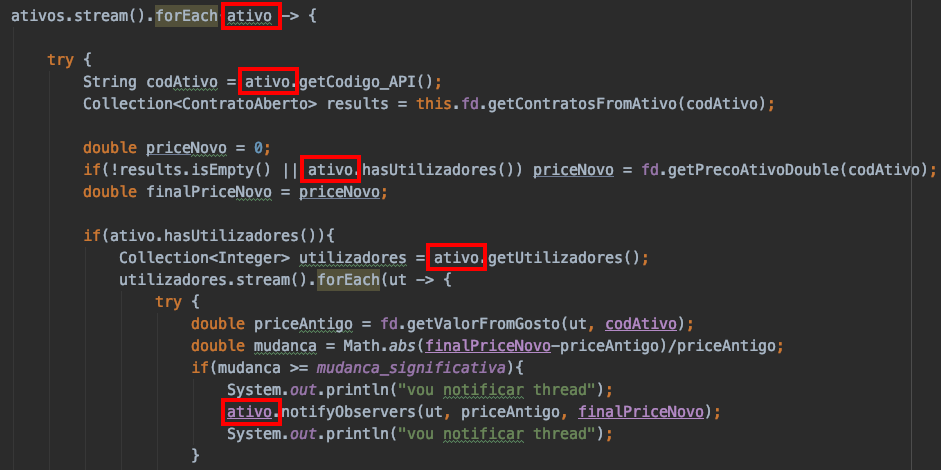
\includegraphics[scale=0.55]{images/change_variable_name_after_2.png}
	\caption{Modificação do nome para ativo.}
	\label{img:pag}
\end{figure}

\chapter{Métricas}
\hspace{5mm} Neste capítulo aborda-se o conjunto de métricas de código que possam ter impacto nas alterações estruturais do código.

\section{Média do número de argumentos}

\hspace{5mm} A métrica proposta pelo grupo, contabiliza a média de argumentos dos métodos alterados pelo \emph{refactoring}. Desta forma, os métodos alterados foram:

\begin{itemize}
    \item notifyObservers() da classe \textbf{Ativo} no package \textbf{Models};
    \item update() da classe \textbf{Facade} no package \textbf{Negócio};
    \item addContratoPortfolio() da classe \textbf{Facade} no package \textbf{Negócio};
\end{itemize}{}
\hspace{5mm}

\begin{table}[H]
    \centering
    \begin{tabular}{|c|c|c|}
    \hline
        método alterado & \# args antes & \# args depois \\ 
        \hline 
        notifyObservers & 4 & 1 \\ 
        \hline
        update & 4 & 1 \\ 
        \hline
        addContratoPortfolio & 9 & 4 \\ 
        \hline
        \hline
        total de argumentos & 17 & 6 \\
        \hline
        média de argumentos & 5.67 & 2 \\
        \hline
    \end{tabular}
    \caption{Número de argumentos antes e depois do \textit{refactoring}.}
    \label{tab:testeFront}
\end{table}

\hspace{5mm} Observando a amostra conclui-se que houve uma \textbf{redução de 64.73 \%} do número de argumentos após o \textit{refactoring}.

\section{Média do número de linhas por método}
\hspace{5mm} A métrica proposta pelo grupo, contabiliza a média do número de linhas por método alterado pelo \emph{refactoring}. No entanto, apenas um método sofreu essa redução, o \textbf{run} da classe \textbf{DealChecker}, no package \textbf{Negócio}.

\hspace{5mm} Inicialmente o método \textbf{run} tinha sessenta e sete linhas, após \emph{refactoring}, passou para onze linhas. Assim, concluí-se que houve uma redução de 83.58 \%.

\section{Número de classes \& interfaces alteradas}
\hspace{5mm} A métrica proposta pelo grupo, contabiliza o número de classes alteradas pelas técnicas de \emph{refactoring}. 

\hspace{5mm} Desta forma, foram alteradas todas as classes \textbf{DAO}, devido a um \emph{code smell} identificado no capítulo anterior, sendo cinco classes. 

\hspace{5mm} Do mesmo modo, no package \textbf{Models}, foram alteradas duas interfaces, \textbf{Observer} e \textbf{Subject} e duas classes, \textbf{Ativo} e \textbf{Utilizador}. 

\hspace{5mm} No package \textbf{Negócio}, foram alteradas as duas classes, \textbf{DealChecker} e \textbf{Facade}. 

\hspace{5mm} Assim, contabiliza-se a modificação de onze classes/interfaces, podendo ter sido mais, caso fosse feito \emph{refactoring} a todo o código.

\hspace{5mm} Note-se que, esta métrica torna-se importante, para concluir, que a arquitetura foi bastante alterada.

\section{Número de design patterns alterados}

\hspace{5mm} A métrica proposta pelo grupo, contabiliza o número de \emph{desing patterns} alterados ou mesmo completamente modificados devido à incorreta implementação dos mesmos.

\hspace{5mm} Desta forma, tal como referido no capítulo anterior, modificou-se os \emph{design patterns} Observer e Factory para a classe \textbf{Ativo}.

\hspace{5mm} Tal como a métrica anterior, esta métrica tem bastante relevância, uma vez que, a alteração de \emph{design patterns} exige sempre muitas alterações na estrutura do código. No caso do \emph{desing pattern} \textbf{Factory}, tal como referido no capítulo anterior, o \emph{refactoring} torna-se mais dispendioso, do que implementar de raiz o próprio \emph{desing pattern}.